

%\documentclass[a4paper]{book}
%\usepackage{mining}
%\begin{document}


\section{mbonsai Decision Tree Generated from Sequence Data \label{sect:mbonsai}}
\index{mbonsai@mbonsai}
This command builds a decision tree model based on sequence patterns. Analysis of the sequence data can be applied in a variety of applications such as order of brands purchased by customers, sales floor cyclic patterns in department stores and supermarkets, the onset order of injuries.  The original idea of this command, BONSAI\cite{SSS94}, was developed by a research team from Kyushu University and Kyushu Institute of Technology. This technique is applied for the analysis of amino acid sequences in molecular biology. Similarly, this command implemented several improvements for the application of sequence analysis in business data with the following features.

\begin{itemize}
 \item Transform patterns from numerical and categorical sequence data into classication conditions.
 \item Use alphabet indexing as data reduction technique for sequence data.
 \item Process multiple variables of sequence data, numerical and categorical variables as predictors.
 \item Allow cost sensitive learning approach to account for dierential misclassification costs.
 \item Allow separate training and testing of decision tree models.
 \item Allow two or more classes in target variable for classification.
 \item Allow cross-validation for assessing performance of predictive model.
\end{itemize}

First, the example below illustrates how to obtain an intuitive understanding of this command. A data set contains purchase sequences of brand \verb|a,b,c| by customers from a retail  store, and the corresponding churn status of the customer is shown in Table \ref{tbl:mbonsai_inp1}. Under the hypothesis of which purchase order of the brand is related to the estrangement of the customer, we will build a decision tree model with partial pattern of brand purchasing order as explanatory variable, and the churn status as target variable (Refer to the next section on details of the definition of patterns that is considered partial string, such as "ab", "cbb").  Pattern used as explanatory variables is referred to as candidate pattern, the pattern generated (More details on this method is available in the next section) will contribute to the accuracy of the model, afterwards, the patterns are converted to 0-1 variable (Table \ref{tbl:mbonsai_inp2}). Decision tree is constructed in a conventional manner from this data set consisting of candidate patterns. The actual decision tree created with this command is shown in Figure \ref{fig:mbonsai_bonsai1}.

\begin{table}[htbp]
\begin{center}
\begin{tabular}{ll}

\begin{minipage}{0.5\hsize}
\begin{center}
\caption{Example of sequence data. Each line corresponds to one customer, with the target variable indicating the status of continual purchase of the customer. The alphabetic characters a, b, c, shown in "BrandSequence"  column represents the brand purchased by the customer in the respective order as shown.
\label{tbl:mbonsai_inp1}}
{\small
\begin{tabular}{lc}
\hline
BrandSequence&Churn \\
\hline
bcaba   & yes \\
bcabcaa & yes \\
aaabac  & yes \\
caa     & yes \\
cca     & no  \\
cacbc   & no  \\
bcc     & no  \\
acca    & no  \\
\hline
\end{tabular} 
}
\end{center}
\end{minipage}

\begin{minipage}{0.5\hsize}
\begin{center}
\caption{The BrandSequence column is extracted from Table \ref{tbl:mbonsai_inp1} and matched against partial purchase patterns as explanatory variables (referred to as candidate patterns). All samples are matched,, the presence of patterns is converted to 0-1 formatted data. In this example, the first record contains the partial pattern "a", "b", "c", "ab" in the sequence, however, “aa” and “cc” is not included. 
\label{tbl:mbonsai_inp2}}
{\small
\begin{tabular}{cccccccl}
\hline
a&b&c&aa&ab&cc&$\cdots$&Churn \\
\hline
1&1&1&0&1&0&& yes \\
1&1&1&1&1&0&& yes \\
1&1&1&1&1&0&& yes \\
1&0&1&1&0&0&$\cdots$& yes \\
1&0&1&0&0&1&& no \\
1&1&1&0&0&0&& no \\
0&1&1&0&0&1&& no \\
1&0&1&0&0&1&& no \\
\hline
\end{tabular} 
}
\end{center}
\end{minipage}

\end{tabular} 
\end{center}
\end{table} 


\begin{table}[htbp]
\begin{center}
\begin{tabular}{ll}

\begin{minipage}{0.5\hsize}
\begin{center}
%\begin{figure}[htpb]
\centering
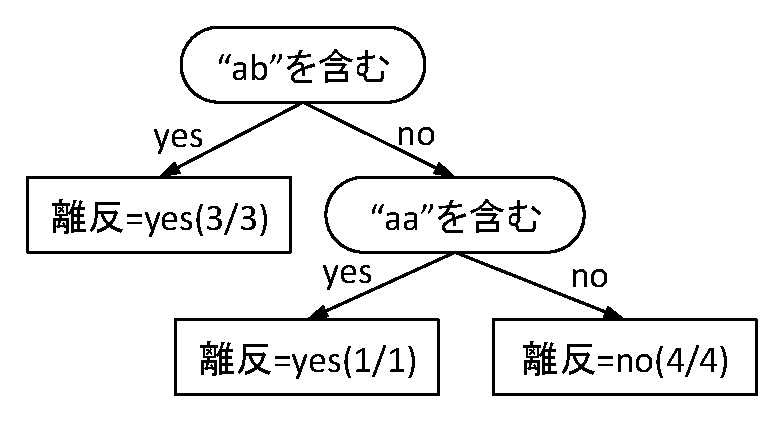
\includegraphics[scale=0.5,clip]{./figure/bonsai1.eps}
\caption{Example of Building Customer Churn Model with BONSAI}
\label{fig:mbonsai_bonsai1}
%\end{figure}
\end{center}
\end{minipage}

\begin{minipage}{0.5\hsize}
\begin{center}
%\begin{figure}[htpb]
\centering
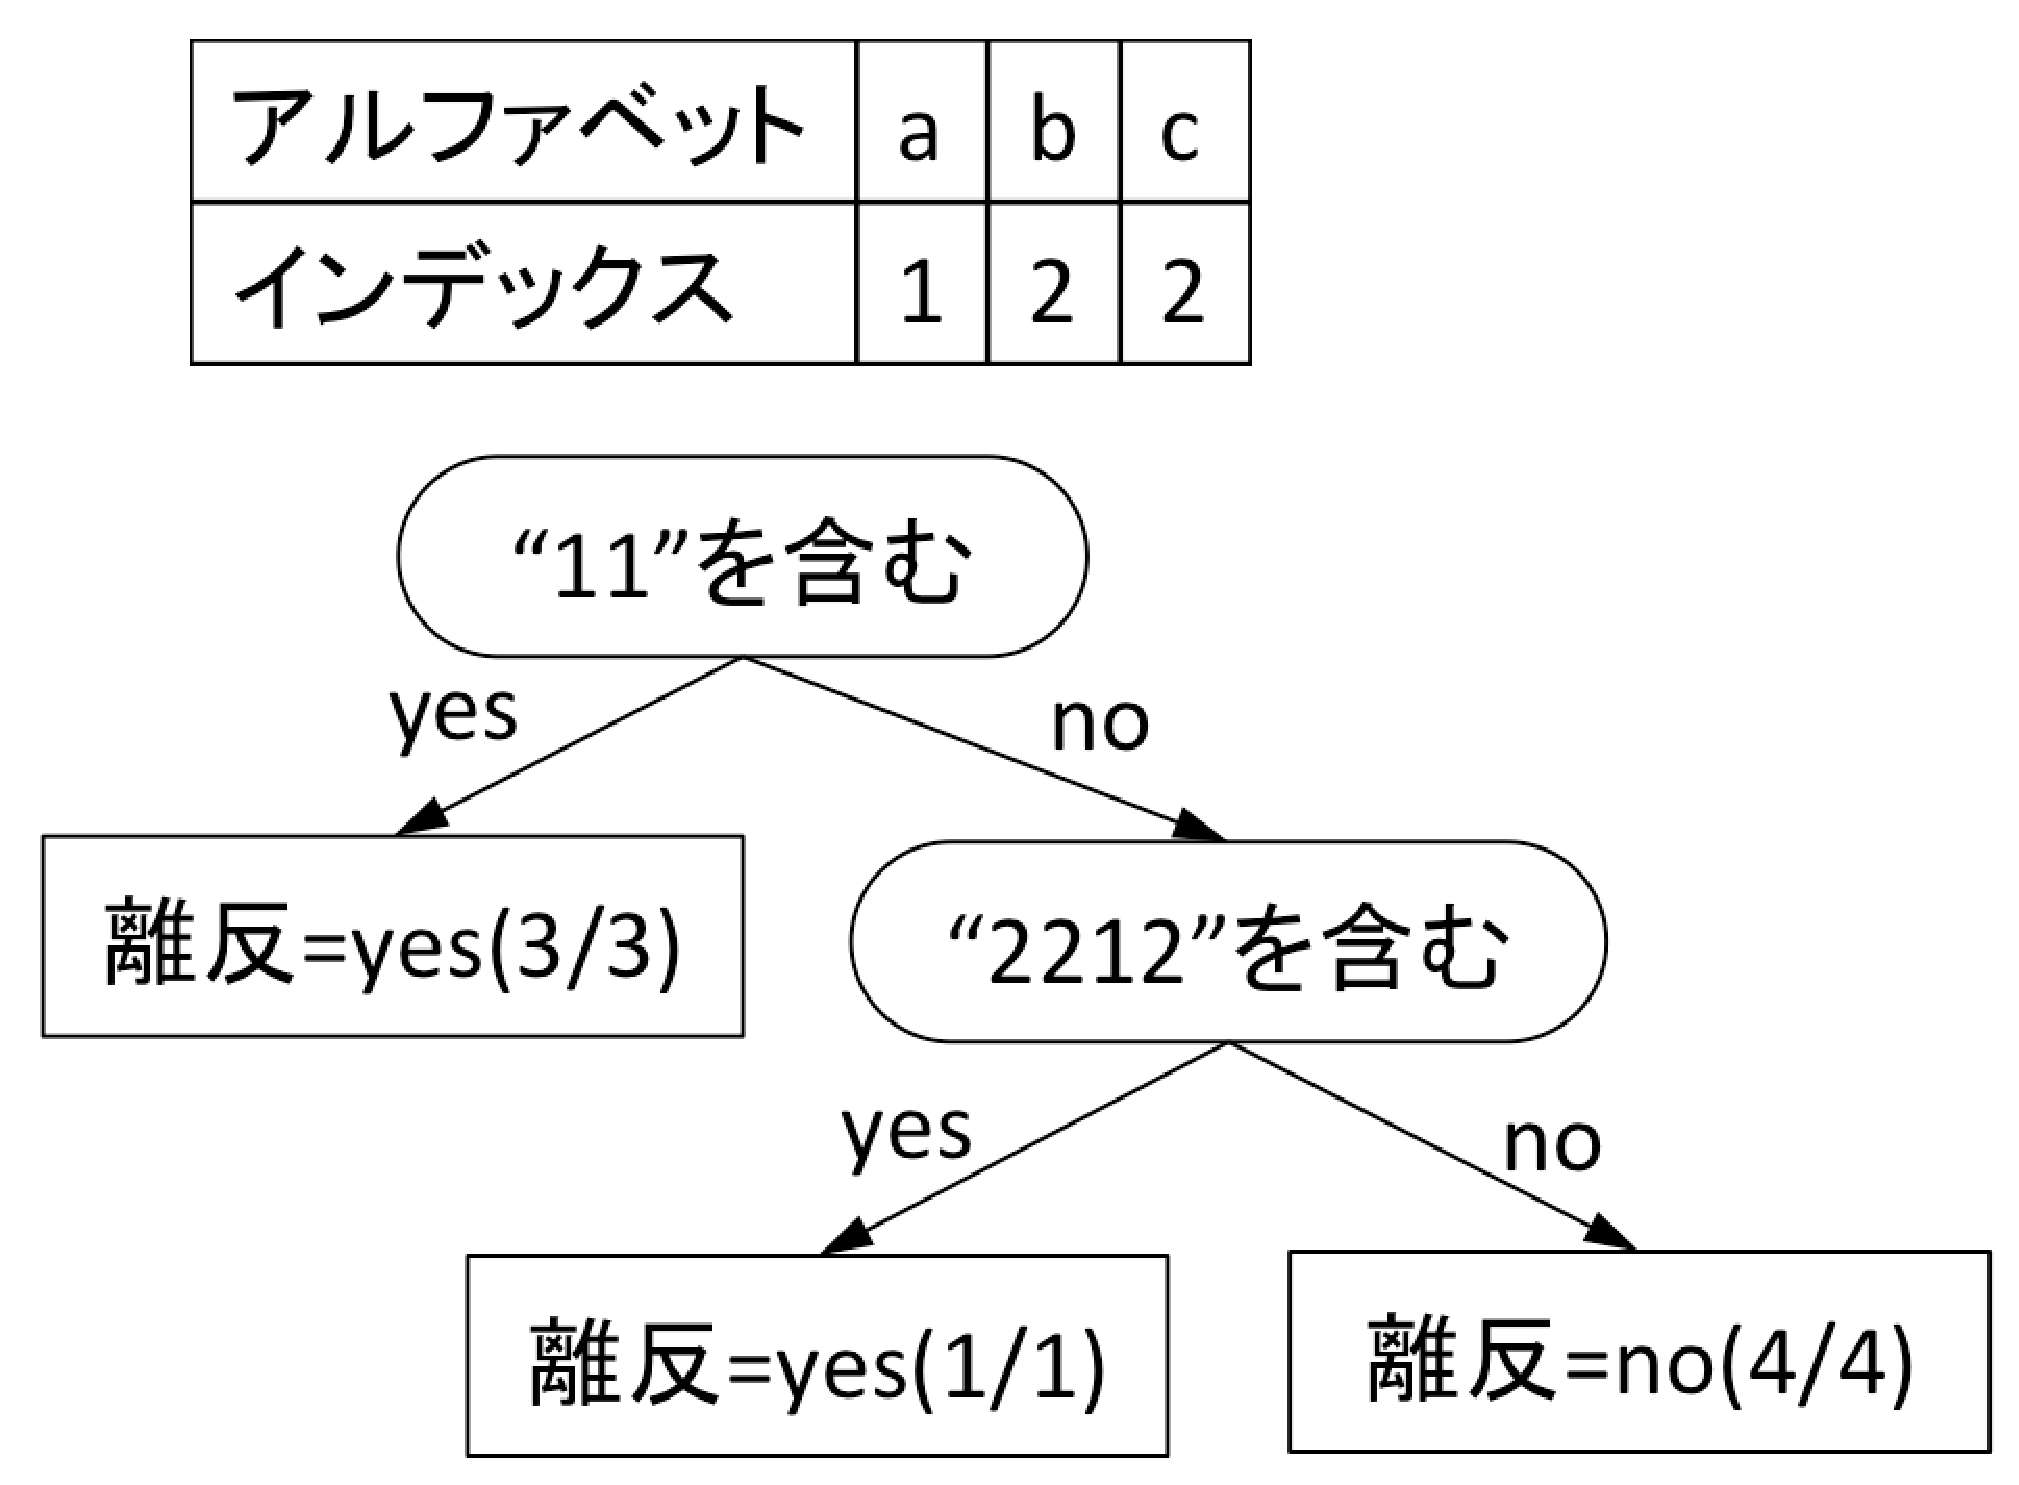
\includegraphics[scale=0.19,clip]{./figure/bonsai2.eps}
\caption{Example of Building Customer Churn Model with BONSAI}
\label{fig:mbonsai_bonsai2}
%\end{figure}
\end{center}
\end{minipage}

\end{tabular} 
\end{center}
\end{table} 

A notable feature of the BONSAI is the function to group elements (known as alphabet) that make up the pattern automatically. The grouping of each alphabet is referred to as index. 

For example, there are three ways to group the 3 brands \verb|a,b,c| into two index (a and bc, b and ac, c and ab), each grouping is replaced with the matching index.  Three decision trees are built with the above described procedure, the best decision tree is selected based on classification accuracy.

Decision tree built in this manner is shown in Figure \ref{fig:mbonsai_bonsai2}. The result of grouping with index increases the accuracy of the classification model, further more, useful knowledge could also be obtained from the result.



\subsection{Details}
The details concerning the construction of the decision tree are explained as follows. 

\subsubsection{Regular pattern }
Given, $n$ character string constants $\pi_1, \pi_2, ..., \pi_n$ on alphabet $\Sigma$, with any of the $n+1$ character string $x_0, x_1, ..., x_n$, regular pattern (also referred to as sequence pattern)  is represented in the format $x_0\pi_1x_1\pi_2x_2 \cdots \pi_nx_n$. This technique is easier to understand when the concept of  wildcard is applied to the field of data retrieval (``*'' is used instead of $x_i$ as wildcard). In this command, besides the definition of regular pattern described above, that is $x_0\pi x_1$, the regular pattern can be handled by restricting to the substring $\pi$ (hereinafter referred to as "string pattern"). The use of string pattern and sequence pattern is specified in the second parameter at \verb|p=|.


\subsubsection{Begin / End Match }
It is possible to specify the matching of beginning and ending string as matching rule for regular pattern of each sample of sequence data. This can be specified in the fourth  (match beginning), and fifth (match ending) parameters of \verb|p=|. Based on this specification, the position of the alphabet of the beginning (or ending) of regular pattern, the beginning (or ending) of sequence data is matched within the specified number of characters. For example, given the sequence data \verb|aabccd|, when matched with character substring pattern \verb|ab| from the left, if the matching sequence only contains 1 character, it is not considered as match, if the beginning of the sequence contains first two characters of the substring pattern, it is considered as match.  If the sequence pattern is made up of \verb|ab|, it is possible to match the first charter in the beginning. If this parameter is not specified, it operates without restriction of matching as described above.



\subsubsection{Alphabetical Order}
This command can deal with order structure that contains alphabets. The key difference of order structure is the rules for creating the index. 
Given the alphabet set $\{a_1,a_2,\dots,a_n\}$, with the relationship of $a_1 \prec a_2 \prec \dots \prec a_n$ for any three consecutive alphabet $a_i,a_{i+1},a_{i+2}$, an index is generated to satisfy the relationship of $\psi(a_i)=\psi(a_{i+2}) \Rightarrow \psi(a_i)=\psi(a_{i+1})$. Here, $\psi(a)$ represents an index to be associated with the alphabet a. This means that the alphabets belonging to a group for indexing must always follow consecutive order. For example,  given three consecutive alphabet $a \prec b \prec c$, $\{a,b\} and \{c\}$ is grouped together, but $\{a,c\} and \{b\}$ is not. Consecutive alphabet can be specified in the third parameter of \verb|p=|. 


\subsubsection{Local Search and Search Space of Optimal Alphabet Index }

Given $n$ number of alphabet(s), the number of cases to be grouped into $m$ or less indexes is not certain, but when $m=2$ is set as limit, the number can be presented in $m^{n-1}$ ways. If both the value of $m,n$ are small, it is possible to construct a decision tree for all cases, and if the value is large, the local search method of searching in subspace is applied. Initially, the random index is set to corresponding alphabet, the corresponding relationship changes bit by bit when building the decision tree, and continue to change until there is no improvements in classification accuracy (Refer to literature \cite{SSS94} for details). Thus, sometimes the results may differ depending on the initial value of the corresponding relationship between the index and the alphabet. In order to obtain the same results from the initial value and select the best model (multi-start),  the initial value can be specified at \verb|iter=| in this command. The default value is \verb|iter=1|.


\subsubsection{Method of Generating Candidate Patterns }
Candidate patterns as shown in Table \ref{tbl:mbonsai_inp2} are generated from the updated alphabet index by local search. The generation of the classification rules for the candidate patterns is based on the nodes of the decision tree. In this command, candidate patterns are enumerated by the heuristics method described below.  First, the index for the regular pattern with length 1 is constructed, and is stored in the priority queue. Precedence in the priority queue is determined by ascending order (see below) of the entropy of a regular pattern Afterwards, select the regular pattern with the lowest entropy in the priority queue, an index is added to the selected regular pattern, regular pattern with length of 2 is created, and stored in priority queue again. Repeat the above steps such that, regular pattern with length $n$ is selected, and regular pattern with length $n+1$ is stored in the priority queue. However,  the index cannot be added when $n$ is greater than 5 (the upper size limit of the regular pattern can be specified in the sixth parameter of \verb|p=|).  In addition, the process will terminate if the size is greater than the number of candidates (specified by \verb|cand=|) specified by the user. Entropy is used to evaluate regular patterns and is also used in the selection of the splitting rules at the nodes of the decision tree, the value of entropy becomes smaller as the regular patterns are classified into extreme distribution classes. Entropy $ent(\pi)$ of regular pattern $\pi$ is defined in Equation \ref{eq:mbonsai_entropy}.


\begin{equation}
ent(\pi)=-q^{{\rm m}(\pi)}\sum_{i=1}^c p_i^{{\rm m}(\pi)} \log p_i^{{\rm m}(\pi)}
            -q^{{\rm u}(\pi)}\sum_{i=1}^c p_i^{{\rm u}(\pi)} \log p_i^{{\rm u}(\pi)}
\label{eq:mbonsai_entropy}
\end{equation}

Here, $c$ represents the number of classes, $p_i^{{\rm m}(\pi)}$($p_i^{{\rm u}(\pi)}$ represents the composition ratio of class $i$ that matches (or unmatch) with the sample in the regular pattern $\pi$ expressed as ($\sum_i^c p_i^{{\rm m}(\pi)}=1$). In addition, $q^{{\rm m}(\pi)}$($q^{{\rm u}(\pi)}$) represents the composition ratio of matching (or unmatch) with regular patterns $\pi$ out of all samples ($q^{{\rm m}(\pi)}+q^{{\rm u}(\pi)}=1$).
 

\subsubsection{Other Types of Variables}
In this command, besides sequence data, numerical and categorical variables can be specified as an explanatory variable. By doing so, it is possible to construct decision tree rule that includes regular patterns with categorical and numerical rules. The creation of branch rules based on category and numbers is similar to that in C4.5 \cite{Quinlan93}. In this command, columns with sequence, numeric, and categorical data can be defined at \verb|p=,n=,d=| parameters. 


\subsubsection{Selection of Splitting Rule }
This command adopts a top down greedy method for the splitting of branches.  In other words, splitting rules at the node of the tree is determined according to the evaluation criteria from the information in the node. The evaluation criteria is based on the selection of branching rules which maximizes the entropy gain. For samples that have been classified into certain nodes, the probability (composition ratio) of class $i$ is represented by $p_i$, the entropy at node is calculated by $ent=-\sum_{i=1}^c p_i \log{p_i}$.  At node $p_i$, number of samples $n$ are classified into class $i$, the ratio of classified sample $n_i$ can be calculated by $n_i/n$. Equation \ref{eq:mbonsai_entropy} shows the entropy gain from the difference of entropy $ent(\pi)$ after splitting the regular pattern $\pi$. It means by splitting the regular pattern $\pi$, how much entropy is reduced. The procedure is repeated until all samples are classified into respective classes at the node, and the tree can no longer be grown bigger.  This type of decision tree is referred to as maximal tree.


\subsubsection{Pruning}
Construct a maximum tree $T_{max}$ according to the method shown in the previous section, but since  the tree size is larger than normal tree, the training data tends to overfit the model, where the classification accuracy of training data is high (misclassification rate decreases), but prediction accuracy of test data decreases. In order to avoid this problem, a small section (including the root node) of the maximal tree is removed during pruning that may be based on noisy or erroneous data. 

In consideration to the set of nodes $t$ from decision tree $T$, where the maximal tree is denoted by $T_{max}=\{t_1,t_2,\dots,t_k\}$, node $t$ and root node of the subtree  is represented by $T_t$, the subtree of node $t\in P$ to root node is pruned (replaced with leaf node) from the decision tree expressed as $T_{max}-\bigcup_{t\in P} T_t + P$. The misclassification rate of decision tree $T$ is denoted by $R(T)$, the pruning is based on the selection of subtree $T^*$ with the lowest misclassification rate on unknown data. It is not possible to determine the actual misclassification rate for unknown data of $T$, instead, it is estimated based on the training data. Given the prediction amount is $C(T)$, the formula of pruning is expressed in the formula \ref{eq:pruning}. 


\begin{equation}
\argmin_{P\subseteq T_{max}} C(T_{max}-\bigcup_{t\in P} T_{t} + P)
\label{eq:pruning}
\end{equation}

To solve this problem, this command applies the cost-complexity pruning method \cite{Breiman84}. This method is comprised of two key phases. First, a series of subtrees $T_1 \supset T_2 \supset \dots \supset T_k$ is selected which is nested from the maximal tree build from the training data (here $T_1$ is the maximal tree, $T_k$ is the root node). Next, the accuracy of these trees is estimated by test sample using cross-validation, the tree with highest prediction accuracy is selected.  

When selecting the series of subtree, the evaluation function of decision tree $T$ measuring the cost complexity is defined as $R_{\alpha}(T)=R(T)+\alpha|\tilde{T}|$, the decision tree model is considered better if the value is smaller. This equation is obtained by balancing the misclassification rate of decision tree $R(T)$, and the tradeoffs of decision tree complexity $|\tilde{T}|$ (number of leaf nodes in $T$) where the complexity parameter is $\alpha(\ge 0)$. In the training data, when the tree size grows larger, the misclassification rate $R(T)$ decreases monotonically, and yet, the complexity $|\tilde{T}|$ increases monotonically. When $\alpha$ is adjusted, the priority of misclassification rate and complexity is also adjusted accordingly. Here, $\alpha$ is fixed as a single value, the pruning process find the subtree $T(\alpha)$ that minimizes the function $R_{\alpha}(T)$. Further, $T(\alpha)$ continues to minimize the tree when $\alpha$ increases, it is possible to enumerate $\alpha$ corresponding to $T(\alpha)$, as a result, the nested subtree $T_1 \supset T_2 \supset \dots \supset T_k$ is created (Refer to \cite{Breiman84} for more details).  Here, the subtree $T_i$ consist of the smallest size decision tree with the minimal cost complexity $\alpha \in (\alpha_i,\alpha_{i+1}]$ .  In the above series of nested subtree, the corresponding cost complexity parameter $\alpha_1,\alpha_2,\dots,\alpha_k$ can be obtained. 

Next, among the series of subtree obtained from the above method, select the optimal subtree $\hat{T}^*$ with the minimum prediction misclassification rate when applied to unknown data. In this command, users can select between test sample method (specified by \verb|ts=|) or cross-validation (specified by \verb|cv=|). In test sample method, training data $D$ is partitioned into two sets  $D_1,D_2$ at a ratio of$1:2$. Then, the maximal tree based on $D_2$ training data is built, based on the complexity parameter $\alpha_1,\alpha_2,\dots,\alpha_k$ obtained from the previous phase, the corresponding subtree is selected. From this subtree, $D_1$ is used as the set of unknown data to predict the value of misclassification rate.  In cross-validation method, training data $D$ is partitioned equally into $n$ sets as $D_1,D_2,\dots,D_n$. First, $D_1$ is treated as unknown data for prediction, similarly, this applies to other training data using the test sample method. Similar process is applied $n$ times to the remaining test data $D_1,D_2,\dots,D_n$, then all training data $D$ is applied as one set for validation. Thus, the average misclassification rate is obtained by this method. From the results obtained above, complexity parameter  $\alpha_1,\alpha_2,\dots,\alpha_k$ for decision tree $T_1, T_2, \dots, T_k$, the optimal decision tree with the lowest misclassification rate is selected. In addition,  the smallest tree whose estimated mean error rate is within one standard error of the estimated mean error rate of the best tree selected (this is called “1 SE rule”).

Nevertheless, pruning can be done by directly specifying the $\alpha$ value without using the cross-validation or test sample method. A decision tree can be built at high speed without having to process calculations for prediction, but the drawback is that the specified $\alpha$ value is arbitrary. 



\subsubsection{Actual Pruning }
In the model building mode, pruning can be done by specifying any of the parameters \verb|ts=|, \verb|cv=|, \verb|alpha=| in this command. When \verb|cv=| or \verb|ts=| is specified, test data is used for prediction, the model with the minimum misclassification rate is selected. In addition, when \verb|alpha=| is specified, the pruned model corresponding to the specified $\alpha$ value is selected. The selection of the model based on the evaluation of the decision tree model is saved in \verb|model.txt| and \verb|model_info.txt|. However,  regardless of any specification, all $\alpha$ corresponding to the maximal tree is calculated internally, at prediction mode (\verb|-predict|), if \verb|alpha=| is specified, it is possible that  different models are used for prediction.  


\subsubsection{Learning Cost Considerations }
When applying classification model, instead of increasing classification accuracy (percentage of correct answers), there are  many instances when it is useful to minimize the  cost of misclassification. Cost is used when predicting customer churn, there are various considerations when implementing cost sensitivity, such as consideration of the cost of customer who stayed who is predicted as customer who left. Construction of model that takes misclassification costs into consideration is known as cost sensitive learning. Various methods have been proposed, the method proposed by Breiman et al \cite{Breiman84} is used in this case. This method is used for the calculation of the branch rule, probability $p_i$ of class $i$ in the sample is therefore modified by assigning cost calculation. Now, the cost of class $j$ that is predicted as class $i$ expressed as $c(i|j)$, given the sum of costs of class $i$ is expressed as $\sum_{j}c(i|j)$, weight is added to class $i$ and probability $p_i$ is updated. If the total cost of class $i$ is large, it means the number of samples are inflated (oversampling), sensitive model based on information of class $i$ is built. The class file in CSV format is shown in Table \ref{tbl:mbonsai_cost}, actual class (\verb|real|), the corresponding predicted class (\verb|predict|) and its cost (\verb|cost|) is displayed in the same row. Given the combination of actual class and predicted class is not specified, and the cost file is not defined, when actual class and predicted class is the same, the cost is 0, otherwise, 1 is set. 


\begin{table}[htbp]
\begin{center}
\begin{tabular}{c}

\begin{minipage}{0.7\hsize}
\begin{center}
\caption{Example of specifying the cost in churn model. In first row, the churn class yes in the actual sample is predicted as no, the cost is set to 2. In the second row, when the churn class no is predicted as yes, the cost is set to 5. The column name can be pre-defined, but must be arranged in the order of actual class, predicted class, and cost. 
\label{tbl:mbonsai_cost}}
{\small
\begin{tabular}{llc}
\hline
real&predict&cost \\
\hline
yes & no  & 2 \\
no  & yes & 5 \\
\hline
\end{tabular} 
}
\end{center}
\end{minipage}

\end{tabular} 
\end{center}
\end{table} 

\newpage 
\subsection{Output Data}
The output of various data files from this command are summarized in Table \ref{tbl:mbonsai_out}. 

\begin{table}[!htbp]
\begin{center}
\begin{tabular}{ll}

\begin{minipage}{1.0\hsize}
\begin{center}
\caption{List of output data from model building mode in mbonasi\label{tbl:mbonsai_out}}
{\small
\begin{tabular}{ | l p{7cm} | p{7cm} |}
\hline
File name&Content&Remarks\\
\hline
\verb|model.pmml|       & The decision tree model represented by PMML\footnote{
Predictive Model Markup Language is an industry standard to describe data mining and mathematical models represented in XML-based file format. Note that this specific command uses an extended tag of the PMML standard.
}                                                 & Records pruning information for maximum tree. \\
                          &                                          & Prediction mode is selected when \verb|-predict| is specified.  \\
\verb|alpha_list.csv|     & Other model information of the complexity parameter $\alpha$    & Series of $\alpha$ corresponding to the model such as the size and accuracy of the model.  \\
\verb|model_min.txt|      & Summary of pruned model with  minimum classification prediction error     & Created when  \verb|cv=| or  \verb|ts=| is specified. \\
\verb|model_1se.txt|      & Summary of pruned model with the same 1SE rule      & Created when  \verb|cv=| or  \verb|ts=| is specified. \\
\verb|model.txt|          & Summary of pruned model for the specified $\alpha$ value    & \\
\verb|model_info_min.csv| & Various information of pruned model with  minimum classification prediction error  & Created when  \verb|cv=| or  \verb|ts=| is specified.  \\
\verb|model_info_1se.csv| & Various information of pruned model with the same 1SE rule  & Created when  \verb|cv=| or  \verb|ts=| is specified.  \\
\verb|model_info.csv|     & Summary of pruned model for the specified $\alpha$    & \\
\verb|predict_min.csv|    & The prediction information of pruned model with  minimum classification prediction error  & Created when  \verb|cv=| or  \verb|ts=| is specified.   \\
\verb|predict_1se.csv|    & The prediction information of pruned model with the same 1SE rule   & Created when  \verb|cv=| or  \verb|ts=| is specified.   \\
\verb|predict.csv|        & The prediction pruned model for the specified $\alpha$ & \\
\verb|param.csv|          & List of execution parameters                       & Returns the pair of keyword-value for the specified parameters \\
\hline
\end{tabular} 
}
\end{center}
\end{minipage}

\end{tabular} 
\end{center}
\end{table} 

\paragraph{model.pmml}
Based on the maximal tree of the decision tree created, \verb|complexity penalty| attribute is shown for each node,  the branch will be pruned when $\alpha$ is greater than the value of complexity penalty. Since the maximal tree and pruning information is recorded in PMML, $\alpha$ is specified for the execution of prediction model, it is possible that the corresponding value will be used to predict the decision tree model.  

\begin{Verbatim}[baselinestretch=0.7,frame=single]
              :
<Node id="0" score="yes" recordCount="8" >
    <Extension extender="KGMOD" name="complexity penalty" value="0.500000"/>
              :
\end{Verbatim}


\paragraph{model\_min.txt,model\_1se.txt,model.txt}
Unlike PMML data, a summary of pruned model is saved in text format. The section \verb|[alphabet-index]| shows the alphabet corresponding to the index. In the following example, alphabet \verb|c| corresponds to index \verb|1|, while \verb|b,a| corresponds to index \verb|2|. The branching rule of the pattern shown in the decision tree is indicated by index symbol.

\begin{Verbatim}[baselinestretch=0.7,frame=single]
[alphabet-index]
Field Name: BrandSequence
Index[1]={c}
Index[2]={b,a}
\end{Verbatim}

The section \verb|[decision tree]| shows the decision tree in text format, information such as  model size (the number of leaf nodes) and number of layers of the deepest leaf is shown below the tree.


\begin{Verbatim}[baselinestretch=0.7,frame=single]
[decision tree]
if($BrandSequence has 22)
  then $Churn=yes (hit/sup)=(4/4)
  else $Churn=no (hit/sup)=(4/4)

number of leaves: 2
deepest level: 1
\end{Verbatim}

 The section \verb|[Confusion Matrix by Training]| shows the prediction classification results of decision tree model using training data. In addition, classification table by cost, prediction accuracy by class, overall prediction accuracy is also shown. 

The section \verb|[Confusion Matrix by Estimation]| is shown when \verb|ts=| or \verb|cv=| is specified. The same format applies to \verb|[Confusion Matrix by Training]| section, the result of test data will be shown differently. 

\newpage
\begin{Verbatim}[baselinestretch=0.7,frame=single]
[Confusion Matrix]
## TRAINING DATA ##
## By count
         Predicted As ...
        yes     no      Total
yes     4       0       4
no      0       4       4
Total   4       4       8

## By cost
         Predicted As ...
        yes     no      Total
yes     0       0       0
no      0       0       0
Total   0       0       0

## Detailed accuracy by class
class,recall,precision,FPrate,F-measure
yes,1,1,0,1
no,1,1,0,1

## Summary
accuracy=1
totalCost=0
\end{Verbatim}

Finally, the section \verb|[Selected Alpha]| shows the value of the complexity parameters used for pruning.

\begin{Verbatim}[baselinestretch=0.7,frame=single]
[Selected Alpha]
alpha: 0
\end{Verbatim}


\paragraph{predict\_min.txt,predict\_1se.txt,predict.txt}
The prediction results is added to the training data used for building the decision tree model in CSV format. The prediction results, as described below, output the highest prediction probability in the \verb|predict| column, and the prediction accuracy for each class (\verb|yes| and \verb|no| as shown below). When \verb|ts=| is specified, it returns the prediction results of test data, when \verb|cv=| is specified, it returns the prediction results by all test data using cross validation. In addition, when \verb|alpha=| is specified,  the prediction result of the training data is returned.  


\begin{Verbatim}[baselinestretch=0.7,frame=single]
Brand Sequence,Churn,predict,yes,no
bcaba,yes,yes,1,0
bcabcaa,yes,yes,1,0
aaabac,yes,yes,1,0
caa,yes,yes,1,0
cca,no,no,0,1
cacbc,no,no,0,1
bcc,no,no,0,1
acca,no,no,0,1
\end{Verbatim}

\paragraph{model\_info\_min.csv,model\_info\_1se.csv,model\_info.csv}

These files store the model information in CSV format. The column \verb|nobs| refer to the number of records in training data, \verb|alpha=| refers to the value of pruning complexity parameter, \verb|accuracy,totalCost| refer to the percentage of correct answers in the test model  and the total cost. 


\begin{Verbatim}[baselinestretch=0.7,frame=single]
nobs,alpha,accuracy,totalCost
8,0,1,0
\end{Verbatim}

\paragraph{alpha\_list.csv}
Display the error rate, standard error, error rate±standard error corresponding to the $\alpha$ value of pruning complexity parameter for the pruned decision tree.

\begin{Verbatim}[baselinestretch=0.7,frame=single]
alpha    ,leafSize,errorRate,SE     ,up     ,lo
0        ,102     ,0.0082   ,0.0015 ,0.0098 ,0.0066
8.15e-05 , 98     ,0.0085   ,0.0016 ,0.0101 ,0.0069
9.41e-05 , 91     ,0.0091   ,0.0016 ,0.0108 ,0.0074
0.000124 , 82     ,0.0100   ,0.0017 ,0.0118 ,0.0083
    :       :         :         :       :       : 
0.035669 ,  2     ,0.0878   ,0.0049 ,0.0927 ,0.0828
1.79e+308,  1     ,0.1399   ,0.0060 ,0.1460 ,0.1339
\end{Verbatim}

\paragraph{param.csv}
Various parameter values used when building the model is stored in CSV format.


\subsection{Format 1: Model building mode}
\begin{verbatim}
mbonsai i= [p=] [n=] [d=] c= O= [delim=] [cost=] [seed=] [cand=] [iter=] [cv=|ts=]
        [leafSize=] [--help]
\end{verbatim}

\begin{table}[htbp]
{\small
\begin{tabular}{ll}

\verb|i=|     & : Training data file name \\
\verb|p=|     & : Column name of pattern (multiple fields can be specified)  \\
              & : Specify up to five parameters after the column name, each separated by a colon.  \\
              & : \verb|p=column_name:is:seq:ordered:head:tail:rs| \\
              & : \verb|is|: Size of the index \\
              & : \ \  When the parameter is not specified, an index is not generated, instead, original alphabet of the pattern is used.   \\
              & : \verb|seq|: Type of pattern  \\
              & : \ \ true: Partial sequence pattern \\
              & : \ \ false: Partial string pattern (default) \\
              & : \verb|ordered|: Arrangement in alphabetical order when generating the index. \\
              & : \ \ \ \ (this parameter is ignored when \verb|is| is not specified) \\
              & : \ \ true: Ordered, group alphabet above / below the threshold value. \\
              & : \ \ false: Unordered(default) \\
              & : \verb|head|: Match string or numeric characters from the beginning (default: start of string is not considered for matching)  \\
              & : \verb|tail|: Match string or numeric characters from the end (default: end of string is not considered for matching) \\
              & : \verb|rs|: Upper size limit of regular pattern (default: 5)  \\
\verb|n=|     & : Column name with numerical data (multiple fields can be specified) \\
\verb|d=|     & : Column name with categorical data (multiple fields can be specified) \\
\verb|c=|     & : Column name of class \\
\verb|O=|     & : Output directory name (text, PMML model, and model statistics)  \\
\verb|delim=| & : Delimiter character of pattern (default: empty character, that is 1 byte character is regarded as 1 alphabet)  \\
\verb|cost=|  & : Name of cost file \\
\verb|seed=|  & : Seed of random number (default=-1: time dependent) \\
\verb|cand=|  & : Number of patterns as explanatory variable (default=30,range:1〜256) \\
\verb|iter=|  & : Iterations of local search (default=1) \\
%\verb|prune=| & : 枝刈り度(default=25,範囲:0〜100,この値が小さければ木のサイズは小さくなる) \\
%\verb|treeSize=| & : 決定木のサイズ上限(決定木のサイズはリーフ数で指定する,default:制限なし) \\
%                 & : 枝刈りの過程で生成される一連の$\alpha_i$について、対応する決定木$T_i$のリーフ数が、\\
%                 & : ここで指定した値より大きければ、そのような$\alpha_i$および$T_i$は、出力の対象としない。\\
\verb|leafSize=| & : Lower limit of the number of samples in one leaf (default: no limit)  \\
\verb|alpha=|    & : Specify the degree of pruning. However, when \verb|cv=| or \verb|ts=| is specified, \\
		& this parameter is disabled. Default=0.01.  \\
\verb|ts=|       & : Specify the percentage of test data partitioned using the test sample method. When "\verb|ts=|" is not specified, the default value is set as 0.333.  \\
\verb|cv=|       & : Specify partition of data by cross-validation method. When "\verb|cv=|" is not specified, the default value is set as 10.  \\
                 & : If either \verb|ts=,cv=| is not specified, default value of \verb|alpha=0.01| will be applied.  \\
                 & : Even when \verb|alpha=,ts=,cv=|, is specified, pruning degree of maximum tree is recorded in PMML,   \\
                 & : the value of \verb|alpha| could change in prediction mode. \\
%\verb|-1se|      & : 枝刈りにおいて、1SE(標準誤差)基準を用いる。\\
\verb|--help|    & : Show help \\

\end{tabular} 
}
\end{table} 

\newpage
\subsection{Format 2: Prediction mode}

\begin{verbatim}
       mbonsai -predict i= I= o= [alpha=] [--help]
\end{verbatim}

\begin{table}[htbp]
{\small
\begin{tabular}{ll}
\verb|-predict| & : Operate in prediction mode. This parameter is required for prediction mode. \\
\verb|i=|       & : Input data [required]  \\
                & : The column names must be the same as the columns that was used for building the model.  \\
\verb|I=|       & : Destination directory path for model building mode [required]  \\
                & : File required are as follows. \\
                & :   bonsai.pmml: pmml containing the decision model  \\
\verb|o=|       & : Output file name containing prediction result \\
                & :    The "predict" column is added to the input data in output. \\
                & : Columns must be the same as columns that was used in building the model.  \\
\verb|alpha=|   & : Specify pruning complexity parameter.  \\
                & : Accepts real number greater than 0, as well as the following two symbols with special functions. \\
                & :   min: $\alpha$ value that corresponds to pruned model which minimizes the estimated misclassification rate. \\
                & :   1se: Alpha value that corresponds to the pruned model with the same 1SE rule.  \\
                & :    Designation of the two symbols is effective only when \verb|ts=|  or  \verb|cv=| is specified when building the model.     \\
                & : Default behavior: \\
                & : If  \verb|ts=| or  \verb|cv=| is specified when building the model, \verb|min| is used. \\
                & : If you specify \verb|alpha=| when building the model, the specified value is applied.   \\
\verb|delim=|   & : Delimiter character of pattern (default: empty character, that is 1 byte character is regarded as 1 alphabet)  \\
\verb|--help|   & : Show help \\

\end{tabular} 
}
\end{table} 


\subsection{Examples}
\subsubsection{Example 1  An example of building a model }

In this example, since \verb|ts=,cv=,alpha=| parameters are not specified, pruning is carried out when \verb|alpha=0.01|,  the result is saved to  the file \verb|model.txt|.

\begin{Verbatim}[baselinestretch=0.7,frame=single]
$ more input.csv
BrandSequence,Churn
bcaba,yes
bcabcaa,yes
aaabac,yes
caa,yes
cca,no
cacbc,no
bcc,no
acca,no

$ mbonsai p=BrandSequence:2 c=Churn i=input.csv O=result1

$ more result1/model.txt

[alphabet-index]
Field Name: BrandSequence
Index[1]={a}
Index[2]={b,c}

[decision tree]
if($BrandSequence has 11)
  then $Churn=yes (hit/sup)=(3/3)
  else if($BrandSequence has 2212)
    then $Churn=yes (hit/sup)=(1/1)
    else $Churn=no (hit/sup)=(4/4)

numberOfLeaves=3
deepestLevel&=& 2

[Confusion Matrix by Training]
## By count
         Predicted As \ldots
	yes	no	Total
yes	4	0	4
no	0	4	4
Total	4	4	8

## By cost
         Predicted As \ldots
	yes	no	Total
yes	0	0	0
no	0	0	0
Total	0	0	0

## Detailed accuracy by class
class,recall,precision,FPrate,F-measure
yes,1,1,0,1
no,1,1,0,1

## Summary
accuracy=1
totalCost=0

$ more result1/model.pmml
<?xml version="1.0" encoding="UTF-8"?>
<PMML version="4.0">
  <Header copyright="KGMOD">
    <Application name="mclassify" version="1.0"/>
    <Timestamp>2014/07/20 23:00:13</Timestamp>
  </Header>
  <DataDictionary numberOfFields="2">
    <DataField name="BrandSequence" optype="categorical" dataType="string">
      <Value value="b"/>
      <Value value="c"/>
      <Value value="a"/>
    </DataField>
    <DataField name="Churn" optype="categorical" dataType="string">
      <Value value="yes"/>
      <Value value="no"/>
    </DataField>
  </DataDictionary>
  <TreeModel functionName="classification" splitCharacteristic="binarySplit">
    <MiningSchema>
      <MiningField name="BrandSequence">
        <Extension extender="KGMOD" name="alphabetIndex">
          <alphabetIndex alphabet="b" index="2"/>
          <alphabetIndex alphabet="c" index="1"/>
          <alphabetIndex alphabet="a" index="2"/>
        </Extension>
      </MiningField>
      <MiningField name="Churn" usageType="predicted"/>
    </MiningSchema>
    <Node id="0" score="yes" recordCount="8">
      <Extension extender="KGMOD" name="pruning" value="0.000000"/>
      <True/>
      <ScoreDistribution value="yes" recordCount="4"/>
      <ScoreDistribution value="no" recordCount="4"/>
      <Node id="1" score="yes" recordCount="4">
        <Extension extender="KGMOD" name="pruning" value="0.000000"/>
        <Extension extender="KGMOD" name="patternPredicate" value="substring">
          <SimplePredicate field="BrandSequence" operator="contain">
            <index seqNo="1" value="2"/>
            <index seqNo="2" value="2"/>
          </SimplePredicate>
        </Extension>
        <ScoreDistribution value="yes" recordCount="4"/>
        <ScoreDistribution value="no" recordCount="0"/>
      </Node>
      <Node id="2" score="no" recordCount="4">
        <Extension extender="KGMOD" name="pruning" value="0.000000"/>
        <Extension extender="KGMOD" name="patternPredicate" value="substring">
          <SimplePredicate field="BrandSequence" operator="notcontain">
            <index seqNo="1" value="1"/>
            <index seqNo="2" value="1"/>
          </SimplePredicate>
        </Extension>
        <ScoreDistribution value="yes" recordCount="0"/>
        <ScoreDistribution value="no" recordCount="4"/>
      </Node>
    </Node>
  </TreeModel>
</PMML>
\end{Verbatim}

\subsubsection{Example 2 Predict unknown data with the model from example 1}

This example predict unknown data (using training data and unknown data in the following) based on the decision tree model constructed. The prediction result includes prediction accuracy of each class (\verb|yes,no| column), class name with the highest accuracy (\verb|predict| column) is returned. 

\begin{Verbatim}[baselinestretch=0.7,frame=single]
$ more unknown.csv
BrandSequence
bcaba
bcabcaa
aaabac
caa
cca
cacbc
bcc
acca

$ mbonsai -predict i=unknown.csv I=result1 o=predict.csv

$ more predict.csv
BrandSequence,predict,yes,no
bcaba,yes,1,0
bcabcaa,yes,1,0
aaabac,yes,1,0
caa,yes,1,0
cca,no,0,1
cacbc,no,0,1
bcc,no,0,1
acca,no,0,1
\end{Verbatim}

%\nopagebreak 
\begin{thebibliography}{9}
\bibitem{Bishop2008}
C.M. ビショップ著, 元田浩, 栗田多喜夫, 樋口知之, 松本裕治, 村田昇(編), パターン認識と機械学習(下):ベイズ理論による統計的予測, 13章, pp.323--370, 2008.

\bibitem{Karypis1999}
Karypis, G. and Kumar, V., "A fast and high quality multilevel scheme for partitioning irregular graphs", SIAM Journal on Scientific Computing 20 (1), pp.359--392, 1999.

\bibitem{Karypis1998}
Karypis, G. and Kumar, V., "Multilevel k-way Partitioning Scheme for Irregular Graphs",
Journal of Parallel and Distributed Compupting 48, pp.96--129, 1998.

\bibitem{SSS94}
S. Shimozono, A. Shinohara, T. Shinohara, S. Miyano, S. Kuhara and S. Arikawa,
Knowledge Acquisition from Amino Acid Sequences by Machine Learning System
BONSAI, {\em Trans. Information Processing Society of Japan},
Vol. 35, pp. 2009-2018, 1994.

\bibitem{Quinlan93}
J. R. Quinlan, {\em C4.5: Programs for Machine Learning}, San Meteo: Morgan Kaufmann, 1993.

\bibitem{Breiman84}
L. Breiman, J. Friedman, R. Olshen, C. Stone
{\em  Classification and regression trees},
Wadsworth: Belmont, CA, 1984.

\end{thebibliography}



%\end{document}
%\end

